\documentclass[10pt]{beamer}

\usetheme{m}

\usepackage{amsmath}

\usepackage{url}

\usepackage{booktabs}
\usepackage[scale=2]{ccicons}

\usepackage{pgfplots}
\usepgfplotslibrary{dateplot}

\usepackage{tikz}
\usetikzlibrary{positioning,shapes,fit}

\usepackage{minted}

\newcommand{\olexrefine}{\emph{olex2.refine}} 
\newcommand{\Olexrefine}{\emph{Olex2.refine}}
\newcommand{\phenixrefine}{\emph{phenix.refine}}
\newcommand{\cctbx}{\emph{cctbx}}
\newcommand{\cctbxrestraints}{\emph{cctbx.restraints}}
\newcommand{\iotbx}{\emph{iotbx}}
\newcommand{\smtbx}{\emph{smtbx}}
\newcommand{\mmtbx}{\emph{mmtbx}}
\newcommand{\scitbx}{\emph{scitbx}}
\newcommand{\lstbx}{\emph{lstbx}}
\newcommand{\sgtbx}{\emph{sgtbx}}
\newcommand{\gltbx}{\emph{gltbx}}
\newcommand{\eltbx}{\emph{eltbx}}
\newcommand{\uctbx}{\emph{uctbx}}

\newcommand{\partialder}[2]{\frac{\partial #1}{\partial #2}}


\title{Constrained Minimisation}
\subtitle{and getting dirty with the CCTBX}
\date{\today}
\author{Luc J. Bourhis}
\institute{Durham University, UK and Bruker AXS}
\titlegraphic{\begin{minipage}{.5\textwidth}
\includegraphics[height=1.5cm]{Bruker_logo.jpg}\end{minipage}
\begin{minipage}{.5\textwidth}
\includegraphics[height=1.5cm]{Durham_University_logo.png}\end{minipage}}

\begin{document}

\maketitle

%\section{CCTBX Map}

\begin{frame}[fragile]
\frametitle{The mathematical problem}
\begin{itemize}
\item We have a structure with $n$ parameters to refine:\\site $x$'s, displacement tensors $U$'s, etc
\item Let's denote the vector of them as $X$
\item Refinement is the minimisation of a function $T(X)$ by varying $X$
\begin{itemize}
\item likelihood in macro-molecular crystallography
\item least-squares in small molecule crystallography
\end{itemize}
\item $X$ can vary continuously
\item So we use methods based on derivatives of $T(X)$ wrt $X$\\ Notation: $\partialder{T}{X}=\left(\partialder{T}{X_1}, \cdots, \partialder{T}{X_n}\right)$
\end{itemize}
\end{frame}

\begin{frame}[fragile]
\frametitle{The mathematical problem}
\begin{itemize}
\item Often we want to restrict $X$ to vary in a limited domain
\item example: --CH3 
\begin{itemize}
\item Position of each Hydrogen = function of position of 
\end{itemize}
\end{itemize}
\begin{flushright}
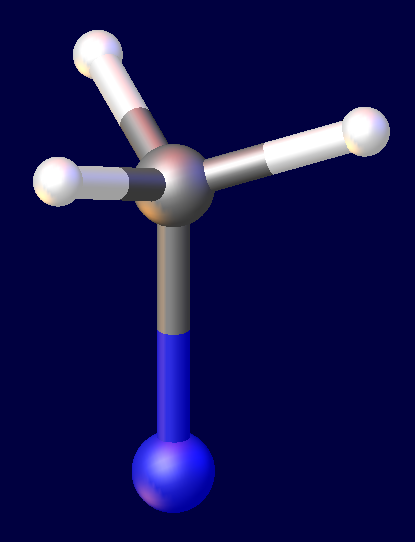
\includegraphics[height=3.5cm]{ch3.png}
\end{flushright}

\end{frame}
\end{document}

